% -*- mode:latex; mode:flyspell -*-
%%%%%%%%%%%%%%%%%%%%%%%%%%%%%%%%%%%%%%%%%%%%%%%%%%%%%%%%%%%%%%%%%%%%%%%%%%%%%%
\section{Correcting relative tracker-calorimeter timing offset}

In an event which has a calorimeter cluster matching to a reconstructed track, the
cluster is included into the track fit as an additional hit. The algorithm reconstructing 
straw hits in the tracker and the algorithm reconstructing the waveform timing in the calorimeter
could add different timing offsets to the reconstructed hits and clusters correspondingly.
Those offsets need to be calibrated out.

A cluster is included into the track fit with the coordinate error $\sigma_{XY} = 15$ mm
and the timing error $\sigma_T = 0.5$ ns.

The distribution of the calorimeter cluster timing residuals for conversion electrons and default Kalman fit 
configuration is shown in Figure \ref{fig:track_cluster_dt}.a. The distribution of cluster timing residuals 
is centered at about -1.17 ns and has a width of about 0.34 ns, indicating presence of the systematic effect.

To study the effect and avoid biasing the fit, the errors assigned to the cluster were increased to $10^6$ (ns or mm),
the corresponding distribution in timing residuals is shown in Figure \ref{fig:track_cluster_dt}.b. 
In this case, inclusion of the cluster into the track fit doesn't bias the result of the fit and one can conclude 
that there is a systematic timing offset between the tracker and the calorimeter, which value is about 1.6 ns.

Figure \ref{fig:track_cluster_dt}.c corresponds to the fit configuration with the cluster time corrected by 1.6 ns, 
and still large errors, and one can see that the applied correction zeroes the timing offset.

Distribution of timing residuals with the cluster time corrected by 1.6ns and default errors (0.5ns and 15mm) 
assigned to the cluster shows a systematic shift of about 0.5-0.6ns, apparently introduced by the fitting procedure.

For now, we correct the cluster timing and use the default resolutions assigned to the calorimeter cluster 
in the Kalman fit.

Correction of the the global track-to-calorimeter timing offset have been introduced {\bf before} 
the tuning of the calorimeter timing resolution has been completed. The global correction zeroing the offset
of the timing residuals was 1.86 ns, whereas after the tuning, the observed offset value is about 1.6 ns.
Resulting non-accounted for systematic offset of about 0.25 ns is however about x2 smaller than the offset
introduced by the Kalman fitter.

It is also worth noting that the width of the distribution of the calorimeter cluster timing residuals is
approximately 50\% of the error assigned to the cluster. The proportionality stays the same, about 50\% level,  
when the timing error assigned to the cluster varies in the range [0.25 ns, 1 ns]. That is another indication
of a non-compensated systematic effect related to the use of the calorimeter cluster in the Kalman fit.

\begin{figure}[h]
  \hspace{-0.8in}
  \begin{tikzpicture}
    \node[anchor=south west,inner sep=0] at (0,0.) {
      % \node[shift={(0 cm,0.cm)},inner sep=0,rotate={90}] at (0,0) {}
      % \makebox[\textwidth][c] {
      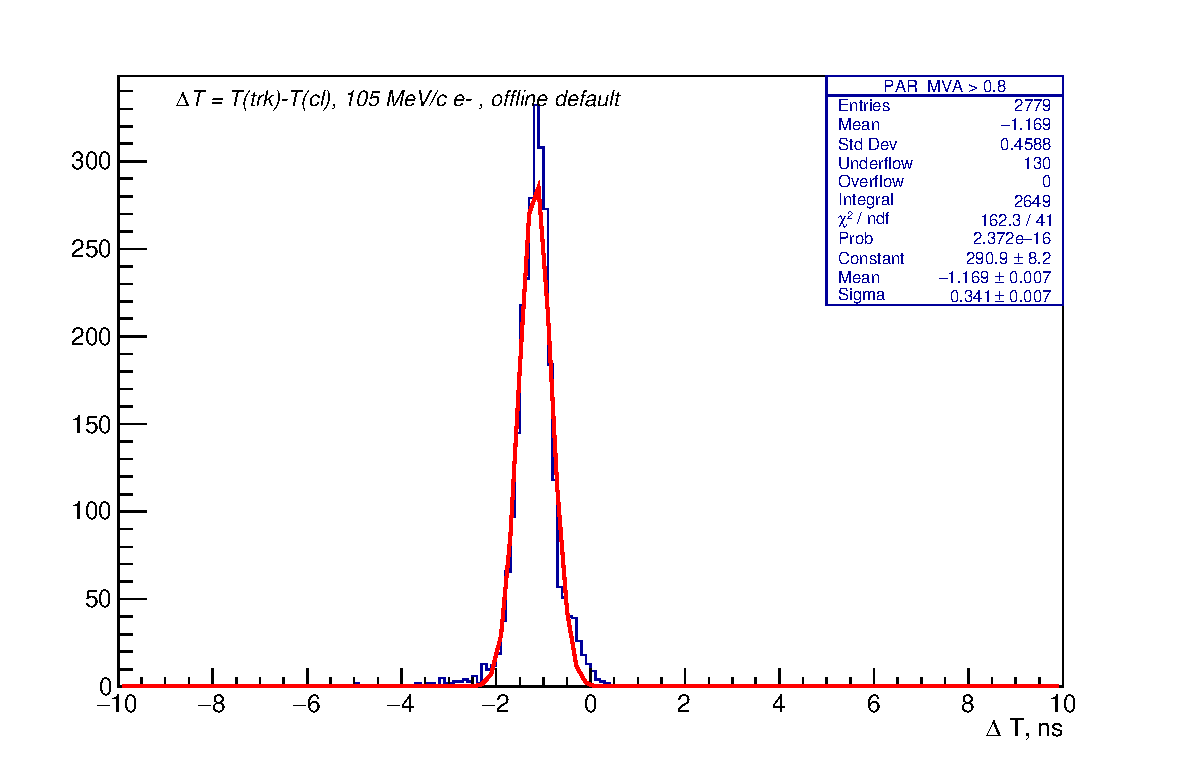
\includegraphics[width=0.64\textwidth]{figures/pdf/figure_00131_ele00s51b0_su2020_track_ana_trk_200_dt}
      % }
    };
    \node [text width=1cm, scale=0.8] at (3.,5) {(a)};
    \node[anchor=south west,inner sep=0] at (10.7,0.) {
      % \node[shift={(0 cm,0.cm)},inner sep=0,rotate={90}] at (0,0) {}
      % \makebox[\textwidth][c] {
      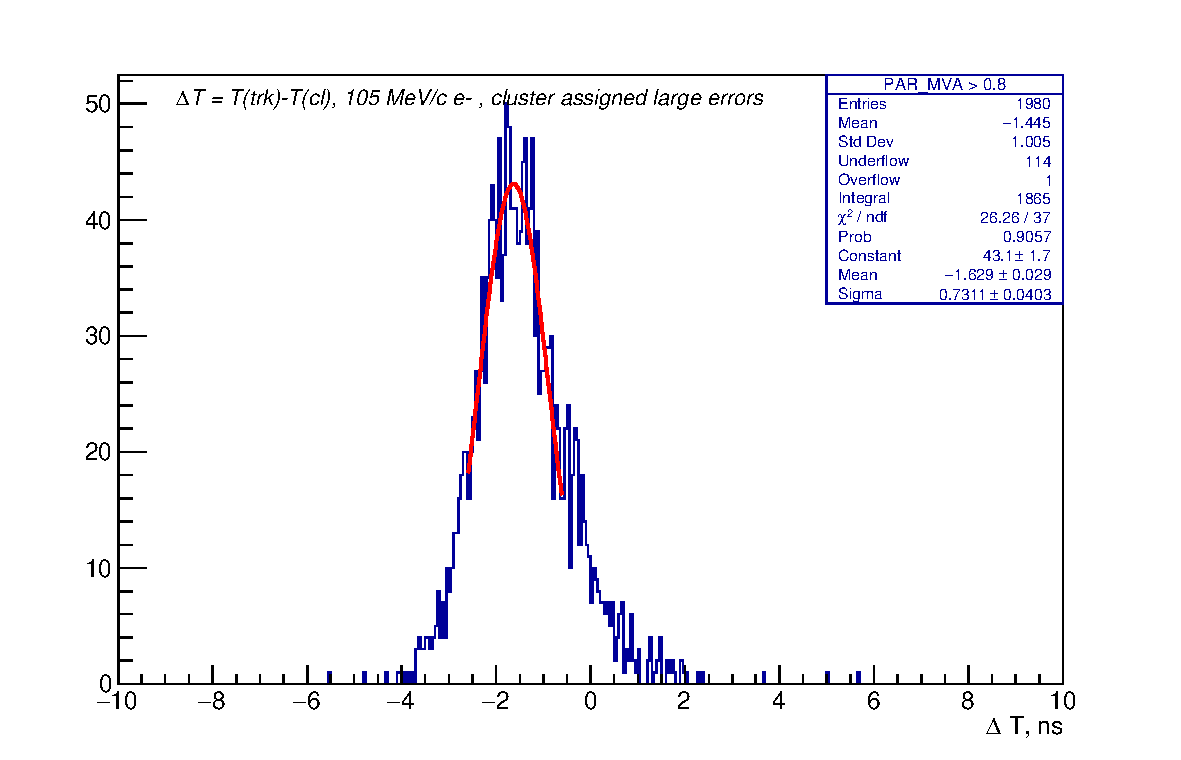
\includegraphics[width=0.64\textwidth]{figures/pdf/figure_00132_ele00s51b0_pid_emuana_trk_101_dt}
      % }
    };
    \node [text width=1cm, scale=0.8] at (13.7,5) {(b)};
    \node[anchor=south west,inner sep=0] at (0,-7.0) {
      % \node[shift={(0 cm,0.cm)},inner sep=0,rotate={90}] at (0,0) {}
      % \makebox[\textwidth][c] {
      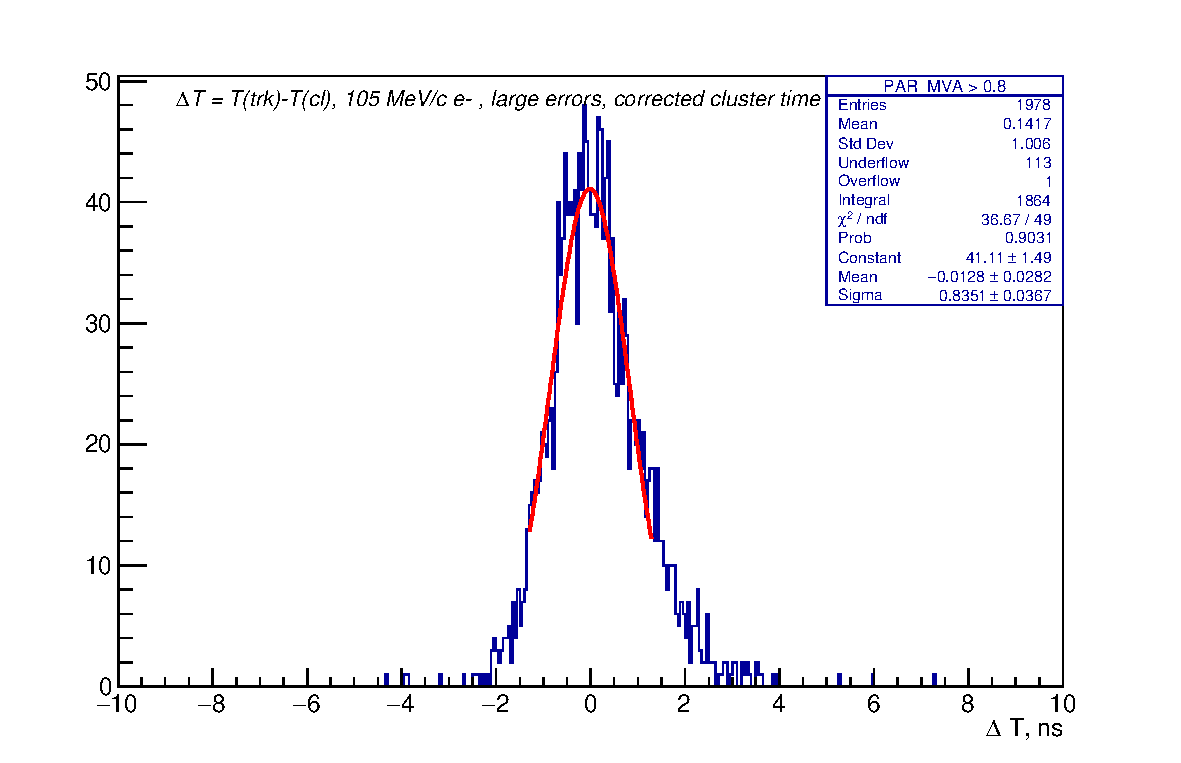
\includegraphics[width=0.64\textwidth]{figures/pdf/figure_00133_ele00s51b0_pid_emuana_trk_101_dt}
      % }
    };
    \node [text width=1cm, scale=0.8] at (3.,-2) {(c)};
    \node[anchor=south west,inner sep=0] at (10.7,-7.0) {
      % \node[shift={(0 cm,0.cm)},inner sep=0,rotate={90}] at (0,0) {}
      % \makebox[\textwidth][c] {
      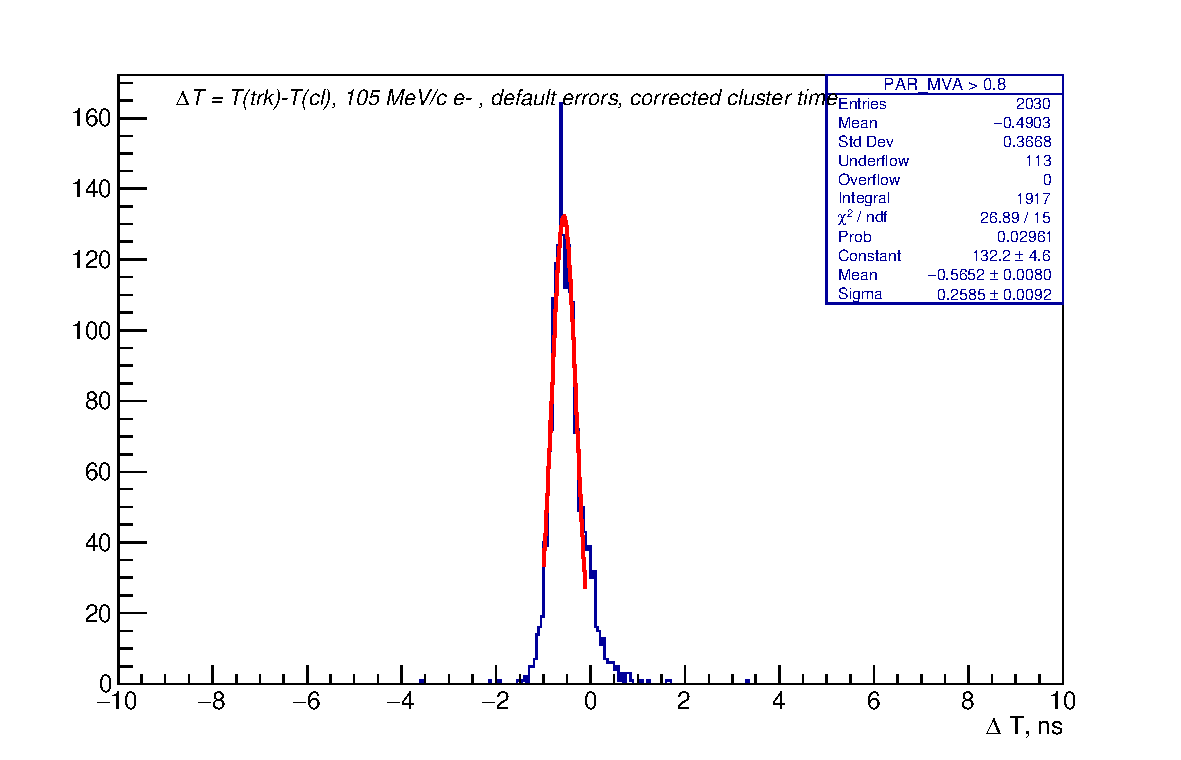
\includegraphics[width=0.64\textwidth]{figures/pdf/figure_00139_ele00s51b0_pid_emuana_trk_101_dt}
      % }
    };
    \node [text width=1cm, scale=0.8] at (13.7,-2) {(d)};
    % \node [text width=6cm, scale=0.8] at (4.5,6.4) {mu2e-18894 by Kevin Lynch and Jim Popp};
  \end{tikzpicture}
  % \captionof{figure} {
  \caption{
    \label{fig:track_cluster_dt}
    Track-cluster timing offsets and their correction: 
    (a) default offline configuration;
    (b) cluster assigned large errors in the fit; 
    (c) cluster timing corrected by 1.6 ns, still large errors;
    (d) cluster timing corrected by 1.6ns, default errors
  }
\end{figure}



%%% Local Variables:
%%% TeX-master: "mu2e-36375"
%%% End:
